\subsection{Memento}
\subsubsection{Định nghĩa}
Memento là một mẫu thiết kế hành vi trong đó một đối tượng được tạo ra để lưu trữ trạng thái của một đối tượng khác và khôi phục lại trạng thái đó sau này mà không tiết lộ chi tiết cài đặt.
\subsubsection{Cách sử dụng}
Memento được sử dụng khi bạn muốn lưu trữ trạng thái của một đối tượng và khôi phục lại trạng thái đó sau này. Điều này có thể xảy ra trong các tình huống như:
\begin{itemize}
    \item Khi bạn muốn lưu trữ một checkpoint hoặc trạng thái tạm thời của một ứng dụng để có thể hoàn tác hoặc khôi phục lại trạng thái trước đó.
    \item Khi bạn muốn theo dõi và lưu lại lịch sử của một đối tượng để có thể quay lại các trạng thái trước đó.
\end{itemize}
\subsubsection{Cấu trúc}
\begin{center}
    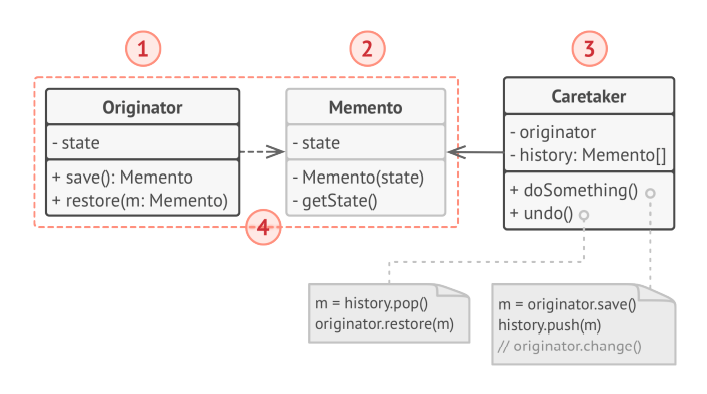
\includegraphics[scale = 0.6]{image/behavioral/memento.png}
\end{center}
\subsubsection{Ưu điểm và Nhược điểm}
Có các ưu điểm và nhược điểm sau:
Ưu điểm:
\begin{itemize}
    \item Nguyên tắc đơn trách nhiệm: Memento chỉ tương tác với nguồn gốc của nó và không gây phụ thuộc đối tượng khác.
    \item Bảo vệ dữ liệu: Dữ liệu bên trong Memento không thể truy cập hoặc sửa đổi từ bên ngoài.
    \item Khi có một số lượng lớn Memento được tạo ra có thể gặp vấn đề về bộ nhớ, performance của ứng dụng.
\end{itemize}
Nhược điểm:
\begin{itemize}
    \item Dùng quá nhiều bộ nhớ: Nếu Memento lưu trữ nhiều trạng thái hoặc đối tượng lớn, nó có thể tiêu tốn nhiều bộ nhớ.
    \item Hiệu suất: Nếu việc tạo và khôi phục Memento quá tốn kém và ảnh hưởng đến hiệu suất chung của ứng dụng.
\end{itemize}
\subsubsection{Code Example}
\begin{itemize}
    \item Có một class Memento chứa level và score.
    \item Một class Game có các phương thức và phải có hàm saveState để giữ trạng thái hiện tại.
    \item Class GameHistory lưu các memento của game.
\end{itemize}
\begin{lstlisting}
#include <iostream>
#include <vector>

// Memento: Represents the snapshot of the state
class Memento {
private:
    int level;
    int score;

public:
    Memento(int level, int score) : level(level), score(score) {}

    int getLevel() const {
        return level;
    }

    int getScore() const {
        return score;
    }
};

// Originator: Creates and restores from mementos
class Game {
private:
    int level;
    int score;

public:
    void playLevel(int level) {
        this->level = level;
        score = 0;
        std::cout << "Playing Level " << level << std::endl;
    }

    void increaseScore(int points) {
        score += points;
        std::cout << "Score increased by " << points << ". Current score: " << score << std::endl;
    }

    Memento saveState() const {
        return Memento(level, score);
    }

    void restoreState(const Memento& memento) {
        level = memento.getLevel();
        score = memento.getScore();
        std::cout << "Restored state: Level " << level << ", Score " << score << std::endl;
    }
};

// Caretaker: Manages the mementos
class GameHistory {
private:
    std::vector<Memento> mementos;

public:
    void addMemento(const Memento& memento) {
        mementos.push_back(memento);
    }

    Memento getMemento(int index) const {
        return mementos[index];
    }
};

int main() {
    Game game;
    GameHistory history;

    // Play Level 1
    game.playLevel(1);
    game.increaseScore(100);
    history.addMemento(game.saveState());

    // Play Level 2
    game.playLevel(2);
    game.increaseScore(150);
    history.addMemento(game.saveState());

    // Play Level 3
    game.playLevel(3);
    game.increaseScore(200);

    // Restore state from Level 2
    game.restoreState(history.getMemento(1));

    return 0;
}

\end{lstlisting}
Ở hàm main, ta thực hiện chơi 3 màn và restore lại màn 2.\\
\newline
\textbf{Kết quả:}
\begin{lstlisting}
Playing Level 1
Score increased by 100. Current score: 100
Playing Level 2
Score increased by 150. Current score: 150
Playing Level 3
Score increased by 200. Current score: 200
Restored state: Level 2, Score 150
\end{lstlisting}
\subsubsection{Các Pattern liên quan}
\begin{itemize}
    \item Két hợp với Command để thực hiện các lệnh hoàn tác.
    \item Kết hợp với Iterator để nắm bắt các trạng thái và thực hiên các lệnh khôi phục.
    \item Hoặc đơn giản chỉ cần ở thời điểm nào đó tạo Clone rồi thời điểm khác lại tạo Clone là ta đã có Memento bản thu nhỏ.
\end{itemize}